% ОБЯЗАТЕЛЬНО ИМЕННО ТАКОЙ documentclass!
% (Основной кегль = 14pt, поэтому необходим extsizes)
% Формат, разумеется, А4
% article потому что стандарт не подразумевает разделов
% Глава = section, Параграф = subsection
% (понятия "глава" и "параграф" из стандарта)
\documentclass[a4paper,article,14pt]{extarticle}

% Подключаем главный пакет со всем необходимым
\usepackage{spbudiploma}

% Пакеты по желанию (самые распространенные)
% Хитрые мат. символы
\usepackage{euscript}
% Таблицы
\usepackage{longtable}
\usepackage{makecell}
% Картинки (можно встявлять даже pdf)
\usepackage[pdftex]{graphicx}

\usepackage{amsthm,amssymb, amsmath}
\usepackage{textcomp}


\begin{document}

% Титульник в файле titlepage.tex
% --------------------- Стандарт СПбГУ для ВКР --------------------------
% Автор: Тоскин Николай, itonik@me.com
% Если заметили ошибку, напишите на email
% Если хотите добавить изменение самостоятельно, GitHub: . PR-s welcome!
% Использованы материалы:
% habr.com/ru/post/144648/
% cpsconf.ru
% Текст:
% http://edu.spbu.ru/images/data/normativ_acts/local/20181030_10432_1.pdf
% Титульный лист:
% http://edu.spbu.ru/images/data/normativ_acts/local/20180703_6616_1.pdf
% -----------------------------------------------------------------------

% Титульный лист диплома СПбГУ
% Временное удаление foot на titlepage
\newgeometry{left=30mm, top=20mm, right=15mm, bottom=20mm, nohead, nofoot}
\begin{titlepage}
\begin{center}
% Первый символ съедается, первым знаком поставлен Ы
\text{Санкт--Петербургский государственный университет}\\
\textbf{Кафедра технологии программирования}

\vspace{22mm}

\textbf{\Large Бельков Роман Андреевич} \\[7mm]
% Название
\textbf{\large Научно-исследовательская практика}\\[12mm]
\textbf{\Large Калибровка рекомендательных систем. Поиск гетерогенного эффекта и нетипичных пользователей для задач рекомендаций контента}

\vspace{12mm}
Направление 01.03.02 \\«Прикладная математика и информатика»\\
Основная образовательная программа СВ.5005.2015
«Прикладная математика, фундаментальная информатика и программирование»\\

\vspace{18mm}

% Научный руководитель, рецензент
% Сходить в уч отдел и узнать, правильно ли
\begin{flushleft}
{\setlength{\leftskip}{23em}
 {Руководитель практики:} \\
 канд. техн. наук, \\
 доцент \\ Блеканов И. С. \\
}
\end{flushleft}

\vfill

{Санкт-Петербург}
\par{2020 г.}
\end{center}
\end{titlepage}
\restoregeometry
\addtocounter{page}{1}


\specialsection{Введение}

В настоящее время, количество информации растет очень быстрыми темпами и чтобы предоставлять наиболее релевантную и полезную для пользователей информацию, 
в веб сервисах начали использовать рекомендательные системы.  Рекомендательные системы обеспечивают персонализированный пользовательский опыт во многих различных областях применения, включая интернет-магазины, социальные сети и потоковое воспроизведение музыки/видео.  
Рекомендательная система -- это алгоритм, который предсказывает наиболее интересные
 объекты для конкретного пользователя на основе некоторой информации о нем.

 Если пользователь посмотрел, 80 артхаусных фильмов и 20 комедий, то вполне разумно ожидать, что персонализированный список рекомендуемых фильмов будет состоять примерно из 80\% артхаусных и 20\% комедий. Это важное свойство, известное как калибровка, недавно получило новое внимание в контексте справедливости машинного обучения. В рекомендуемом списке элементов калибровка гарантирует, что различные области интересов пользователя будут отражены в соответствующих пропорциях. Калибровка особенно важна в свете того факта, что рекомендательные системы, оптимизированные в сторону точности
  в обычном автономном режиме, могут легко привести к рекомендациям, где меньшие интересы пользователя вытесняются основными интересами пользователя.
 В этой статье мы покажем, что рекомендательные системы, обученные точности, могут легко генерировать списки рекомендуемых элементов, которые фокусируются на основных областях интересов пользователя, в то время как меньшие области интересов пользователя, как правило, недопредставлены или даже отсутствуют. 
 Со временем такие несбалансированные рекомендации несут в себе риск постепенного сужения областей интересов пользователя -- что аналогично эффекту пузыря фильтров. Эта проблема также применима в случае нескольких пользователей, совместно использующих одну учетную запись, когда интересы менее активных пользователей в рамках одной учетной записи могут быть вытеснены в рекомендациях.
 Калибровка -- это общая концепция машинного обучения, и в последнее время она переживает возрождение в контексте справедливости алгоритмов машинного обучения. Алгоритм классификации называется калиброванным, если прогнозируемые пропорции различных классов согласуются с фактическими пропорциями точек данных в имеющихся данных. 

\specialsection{Постановка задачи}

Основная цель работы заключается в реализации метода калибровки рекомендательных систем, который бы не сильно ухудшал точность работы рекомендательной системы, но в то же время учитывал все интерес пользователя.
\\

Для достижения цели были поставлены следующие задачи:
\begin{enumerate} 
    \item Обзор существующих методов калибровки рекомендательных систем.
    \item Реализация алгоритма на языке Python.
    \item Поиск или сбор данных и проверка реализованного метода на данных.
  \end{enumerate}
  
\pagebreak
\section{Обзор литературы}
\subsection{Расстояние Кульбака-Лейблера}
В ходе работы был проведен обзор литературы и найдено два метода потенциально подходящих для решения поставленной проблемы. Первый метод заключается в пересчете целевой метрики с помощью расстояния Кульбака-Лейблера (\ref{eq:KL}). \cite{voc1}
\begin{equation}
  C_{KL}(p,q) = KL(p||\tilde{q}) = \sum_g p(g|u)\log\frac{p(g|u)}{\tilde{q}(q|u)},
  \label{eq:KL}
\end{equation}
где ${p}$ это целевое распределение жанра ${g}$ для пользователя $u$, $q$ -- полученное распределение жанров для пользователя.
Во избежание случая $q(g|u)=0$, будем использовать 
\begin{equation}
  \tilde{q}(q|u) = (1-\alpha) \cdot q(g|u) + \alpha \cdot p(g|u)
\end{equation} с очень маленьким $\alpha>0$, такое что $q\approx\tilde{q}$.

Сама же калибровка выполняется по формуле: 
\begin{equation}
  \label{eq:Calibrated}
  I^*=\arg \max_{I, |I|=N} (1-\lambda) \cdot s(I) - \lambda \cdot C_{KL}(p,q(I)),
\end{equation} где $\lambda \in [0,1]$, которая определяет компромисс между расстоянием Кульбака-Лейблера и значением метрики полученным рекомендательной системой. $s(I)=\sum_{i\in I}s(i)$, где $s(i)$ -- степень уверенности, что фильм $i$ подойдет пользователю, предсказанная рекомендательной системой.
\subsection{Метод Сент-Лагю}
Второй алгоритм является адаптацией метода Сент-Лагю. \cite{voc2} Метод Сент-Лагю, был изобретен французским математиком Андре Сент-Лагю для пропорционального распределения мандатов в правительстве. Суть метода заключается в поочередном присуждении мандатов партии с наибольшей квотой, которая на кажом шаге считается по формуле $\frac{V}{2s+1}$, где $V$ -- количесвто голосов, полученных партией, s -- количество мандатов, выделенных партии на данном шаге.

Можно модифицировать данный метод под наш случай. Имея список наиболее релевантных фильмов, мы будем формировать новый список, выбирая фильмы по одному методом Сент-Лагю, только вместо партий у нас будут жанры, а голоса, полученные партией, заменятся на количество понравившихся пользователю фильмов конкретного жанра.
\section{Реализация}
\subsection{Набор данных}
Мною был выбран датасет MovieLens 1M \cite{voc3}, включающий в себя 1 миллион оценок 4,000 фильмов от 6,000 пользователей.
\subsection{Scikit SurPRISE}
SurPRISE \cite{voc4} -- библиотека на языке Python, которая включает в себя реализацию построения и анализа рекомендательных систем. 
Из этого пакета, был использован метод SVD для построения рекомендательной системы.
\begin{figure}[ht]
  \begin{center}
  \scalebox{0.3}{
     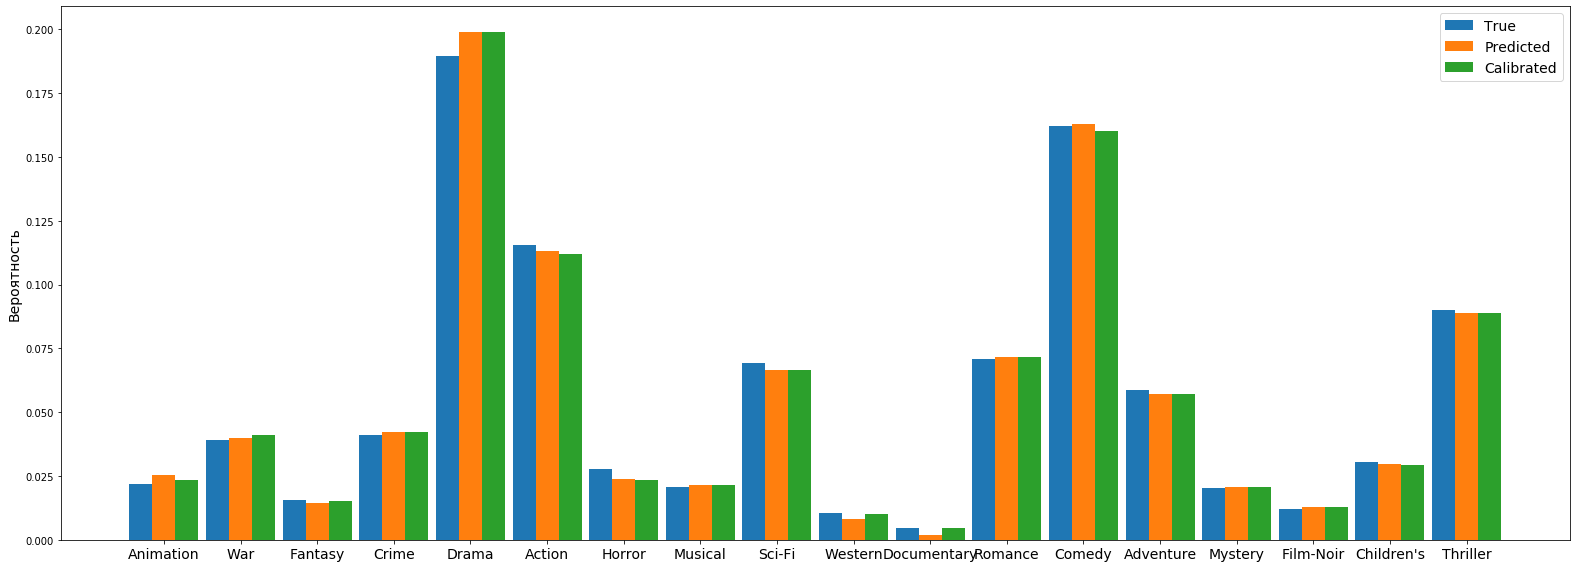
\includegraphics{images/graph.png}
  }
  
  \caption{
  \label{graph-fig}
       Распределение жанров.}
  \end {center}
  \end {figure}
\pagebreak

\subsection{Результаты}
Получив вектор предсказаний, я построил графики реального, предсказанного и откалиброванного распределения жанров фильмов для всех пользователей, они изображены на рисунке \ref{graph-fig}. 
Как видно на графике, распределение, полученное рекомендательной системой, плохо отражает такие жанры, как вестерн и документальное кино, а после калибровки распределение стало ближе к реальному. 
Калибровка была произведена с помощью расстояния Кульбака-Лейблера по формуле (\ref{eq:Calibrated}), с коэффициентом $\lambda=0.2$.


  \pagebreak

% Библиография в cpsconf стиле
% Аргумент {1} ниже включает переопределенный стиль с выравниванием слева
\begin{thebibliography}{1}
\bibitem{voc1} Harald Steck \flqq Calibrated Recommendations\frqq. RecSys '18: Proceedings of the 12th ACM Conference on Recommender Systems, 2018, pp. 154–162, \href{https://doi.org/10.1145/3240323.3240372}{doi.org/10.1145/3240323.3240372}.
\bibitem{voc2} Van Dang and W. Bruce Croft \flqq Diversity by Proportionality: An Election-based Approach to Search Result Diversification\frqq. SIGIR '12: Proceedings of the 35th international ACM SIGIR conference on Research and development in information retrieval, 2012, pp. 65-74, \href{https://doi.org/10.1145/2348283.2348296}{doi.org/10.1145/2348283.2348296}.
\bibitem{voc3} F. Maxwell Harper and Joseph A. Konstan \flqq ACM Transactions on Interactive Intelligent Systems\frqq. ACM Trans. Interact. Intell. Syst. 5, 4, Article 19, 2015, \href{https://doi.org/10.1145/2827872}{doi.org/10.1145/2827872}.
\bibitem{voc4} Nicolas Hug \flqq Surprise a Python library for recommender systems\frqq. 2017, \href{http://surpriselib.com}{surpriselib.com}.
\end{thebibliography}
\end{document}